\documentclass[paper=a4, fontsize=13pt]{article} 
\usepackage[top=1in, bottom=1in, left=1in, right=1in]{geometry}
\usepackage{amstext}
\usepackage{subfigure}
\RequirePackage{graphicx}
\RequirePackage{longtable,multirow,hhline,tabularx,array}
\usepackage[english]{babel} 
\RequirePackage{colortbl,booktabs}
\linespread{1.5}

\title{
\normalfont \normalsize
\huge Battle of Online and Offline Consumption: \\
Comparative Analysis of Amazon and Walmart Stocks
}
\author{Cai Yuzhu, Li Hongchi, Ning Xu, Xue Zheng}
\date{\normalsize\today}

\begin{document}
\maketitle
\section{Introduction}
Online consumption is a relative new and prevailing concept raised in recent decade. Amazon is arguably one of the most successful online firms. As of this writing, its market cap is over \$460 billion, almost twice than the large and well-known offline retailer, Wal-Mart's, with market cap about \$240 billion.

Amazon, as a business model, has many potential advantages relative to a physical operation. It held out the potential of lower inventory and distribution costs and reduced overhead. Consumers could find the books products they were looking for more easily and a broader variety could be offered for sale in the first place. It could accept and fulfill orders from almost any domestic location with equal ease. And most purchases made on its site would be exempt from sales tax.

On the other hand, it is also acknowledged that there are some limitations of online operations. Customers would have to wait for their orders to be received, processed, and shipped. Because they couldn't physically inspect a product before ordering, Amazon would have to make its returns and redress processes transparent and reliable, and offer other ways for consumers to learn as much about the product as possible before buying.
The task to judge the performance of online consumption against offline consumption is compelling. And the methods of judgments comparisons can be diverged. In this term paper, our group conducts time series data models with conditional heteroscedasticity, which are widely applied in financial data analysis, to depict the stock volatility of Amazon and Wal-Mart's.

The historical stock price data presents a diverged trend that seems to reveal a competitive relation between Amazon and Wal-Mart. Admittedly the share price cannot represent complete information about the firms, such as market shares. Nevertheless, this is a direct and prevalent way to evaluate firms' performance through numerical results. And the maximize likelihood method (MLE) estimations will also provide helpful suggestions about their prospective performance.

We organize our discussion as follows. The next section lays out some basic facts about the historical stock price data: statistics and time plots. Section 3 discusses how to determine the specifications of models. Section 4 conducts MLE method to estimate the parameters of models. Section 5 explores future performance and compares our prediction with recent data. A short concluding section follows.

\section{Data Processing}
In our research report, we use Walmart as the representative of offline retail industry and Amazon as that of online retail industry. We focus on the daily log return of Walmart stock and Amazon stock from January 3th, 2010 to December 30th, 2016, with 1761 observations. All the data are pulled from Wind Terminal.

We compute the daily log return based on the  daily close price. Let $r_t$ be the log return of an asset at time $t$, and the formula we use to calculate the log return is
\[ r_t = ln(\frac{p_t}{p_{t-1}}) \times 100\% \]
where $p_t$ is the close price in day $t$ and $p_{t-1}$ is the close price in day {t-1}.

The descriptive statistics and time plots are shown in Table \ref{ds} and Firgure \ref{tp}.

\begin{table}[!htbp]
\caption{Descriptive Statistics}  
\centering  
\subtable[Amazon Stock]
{  
\begin{tabular}{ccccc}
  \toprule
  \rowcolor[gray]{.8}
Year & Sample & Mean(\%) & Sd(\%) \\ 
  \midrule
2010 & 251 & 0.1179 & 2.0591 \\ 
2011 & 252 & -0.0155 & 2.4337 \\ 
2012 & 250 & 0.1484 & 1.9656 \\ 
2013 & 252 & 0.1839 & 1.6947 \\ 
2014 & 252 & -0.0995 & 2.0677 \\ 
2015 & 252 & 0.3089 & 2.0582 \\ 
2016 & 252 & 0.0412 & 1.8682 \\ 
2010-2016 & 1761 & 0.0978 & 2.0323 \\ 
   \bottomrule
\end{tabular}
}  
\qquad  
\subtable[Walmart Stock]
{          
\begin{tabular}{ccccc}
  \toprule
  \rowcolor[gray]{.8}
Year & Sample & Mean(\%) & Sd(\%) \\ 
  \midrule
2010 & 251 & 0.0068 & 0.8782 \\ 
2011 & 252 & 0.0515 & 1.0469 \\ 
2012 & 250 & 0.0627 & 1.0309 \\ 
2013 & 252 & 0.0662 & 0.7749 \\ 
2014 & 252 & 0.0445 & 0.8367 \\ 
2015 & 252 & -0.1229 & 1.3191 \\ 
2016 & 252 & 0.0590 & 1.2030 \\ 
2010-2016 & 1761 & 0.0239 & 1.0297 \\ 
   \bottomrule
\end{tabular}
}
\label{ds} 
\end{table}  

\begin{figure}[!htbp]
\begin{minipage}[!htbp]{0.5\linewidth}
\centering
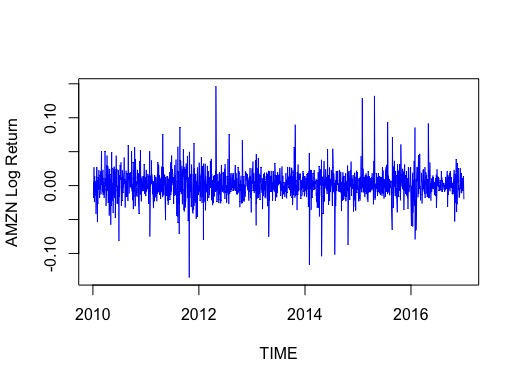
\includegraphics[scale = 0.45]{img/timeplot_AMZN}
\end{minipage}
\begin{minipage}[!htbp]{0.5\linewidth}
\centering
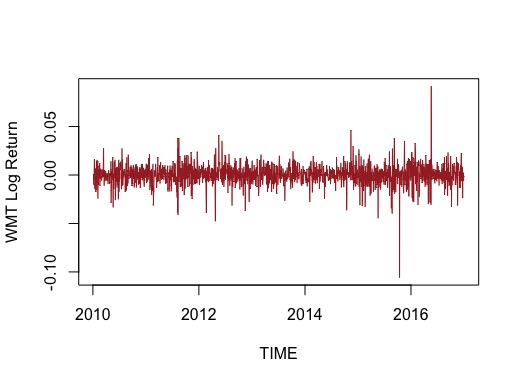
\includegraphics[scale = 0.45]{img/timeplot_WMT}
\end{minipage}
\caption{Timeplots of Amazon (Blue) and Walmart (Red) Stocks}
\label{tp}
\end{figure}

From Table \ref{ds}, we can easily see that both returns of these two stocks display an increasing trend from 2010 to 2016. However, the average log return of Amazon stock  is four times greater than Walmart stock, while the log return of Walmart stock is more stable than Amazon's. From the timeplots in Figure \ref{tp}, the log return series for both stocks appear to be relatively stationary over times, fluctuating around the mean value.

\section{Model Establishment}
\subsection{Model Specification}
First of all, we determine the model to capture the log return fluctuation of Amazon stock. Figure \ref{cf_AMZN}.(a) shows the sample ACF of the log returns, which suggests that there is no significant serial correlations. Figure \ref{cf_AMZN}.(b), showing the sample PACF of the log returns, also confirms our conclusion of no serial correlation. Then, we plot the sample ACF of the squared log returns for Amazon stock in Figure \ref{cf_AMZN}.(c). Combing the three plots, it seems that the log returns are neither serially correlated nor dependent. Similar results can also be found for Walmart stock in Figure \ref{cf_WMT} that the log returns for Walmart stock are serially uncorrelated and independent.

\begin{figure}[!htbp]
\centering
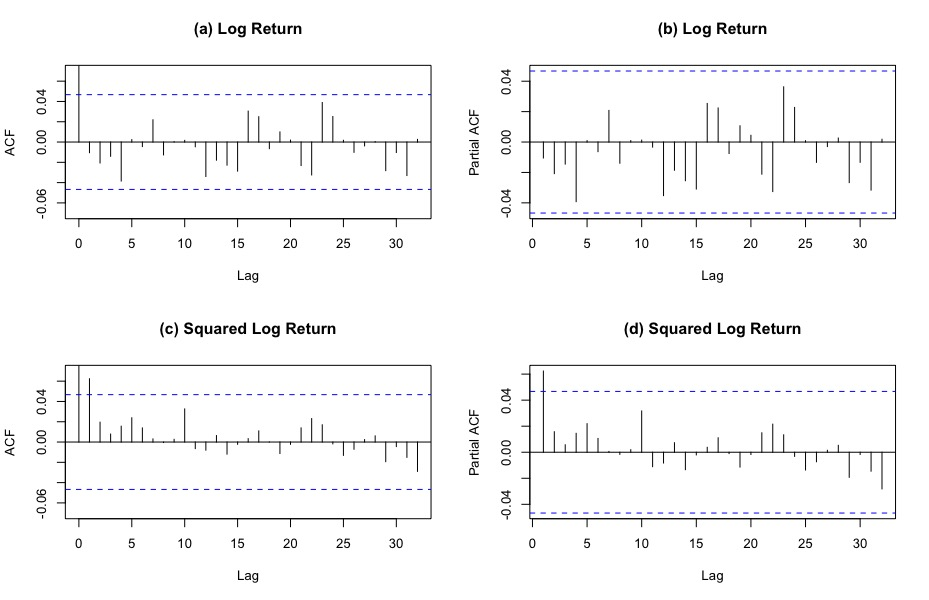
\includegraphics[scale = 0.7]{img/cf_AMZN}
\caption{ACF and PACF of Amazon Stock}
\label{cf_AMZN}
\end{figure}

\begin{figure}[!htbp]
\centering
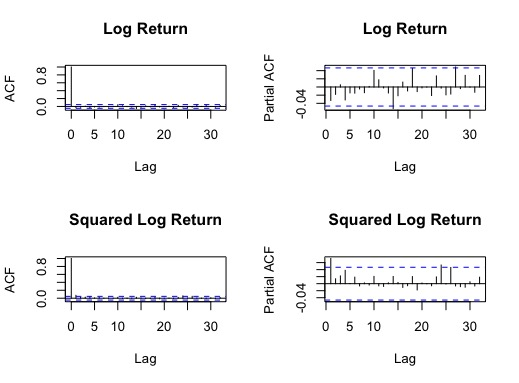
\includegraphics[scale = 0.7]{img/cf_WMT}
\caption{ACF and PACF of Walmart Stock}
\label{cf_WMT}
\end{figure}

\subsection{Mean Equation}
The observations above suggest that the daily log returns of Amazon stock follow an ARMA(0,0) model, in other words, a white noise series. This is in agreement with the result suggested by the sample ACF in Figure 2(c) that all sample ACFs are close to zero. Therefore, we propose a mean equation that is simply a constant plus innovations, $r_t = \mu + a_t$, where $r_t$  is the log return of an asset at time $t$, $\mu$ is the estimate we get using a volatility model. The squared series $a_t^2$ is then used to check for conditional heteroscedasticity (ARCH effects). We perform the usual Ljung–Box statistics Q(m) to the $\{a_t^2\}$ series. The null hypothesis is that the first m lags of ACF of the $a_t^2$ series are zero.

The Ljung–Box statistics of the $a_t^2$ series shows ARCH effects with Q(5) = 9.6519, the p value of which is close to zero.

\subsection{Volatility Equation}
Here we entertain an ARCH(1) model and a GARCH(1,1) model for the volatility and we specify the model as the following:
\[ r_t = \mu+a_t, a_t = \sigma_t \epsilon_t \]
\[ \text{ARCH(1): } \sigma_t^2 = \alpha_0+\alpha_1 a_{t-1}^2 \]
\[ \text{GARCH(1,1): } \sigma_t^2= \alpha_0+\alpha_1 a_{t-1}^2+\beta_1 \sigma_{t-1}^2 \]
in which $\epsilon_t$, here in our model, we assume as a Gaussian innovation that is independent and identically distributed as a Normal distribution with mean 0 and variance 1.

\section{Estimation}

\begin{table}[!htbp] \centering 
  \caption{Ljung-Box tests for ARCH(1) and GARCH(1,1) models for AMZN Stock} 
  \label{} 
\begin{tabular}{cc|cccccc} 
\\[-1.8ex]\hline 
\hline
& & \multicolumn{3}{c}{Standardized residuals} & \multicolumn{3}{c}{Squared standardized residuals} \\
& & Q(10) & Q(15) & Q(20) & Q(10) & Q(15) & Q(20) \\
\hline 
\multirow{2}{*}{ARCH(1)} & statistic & 4.7873 & 10.2395 & 12.8693 & 3.9721 & 4.7376 & 5.1054 \\
& p-value & 0.9049 & 0.8044 & 0.8829 & 0.9486 & 0.9941 & 0.9997 \\
\multirow{2}{*}{GARCH(1,1)} & statistic & 4.1734 & 10.2365 & 12.8473 & 3.0443 & 4.2163 & 4.7107 \\
& p.value & 0.9392 & 0.8046 & 0.8838 & 0.9804 & 0.9969 & 0.9999 \\
\hline
\hline 
\end{tabular} 
\end{table} 

\begin{table}[!htbp] \centering 
  \caption{Results of Estimation of Two Volatility Models for AMZN Stock} 
  \label{} 
\begin{tabular}{@{\extracolsep{5pt}}lcc} 
\\[-1.8ex]\hline 
\hline
 & ARCH(1) & GARCH(1,1) \\ 
\hline \\[-1.8ex] 
 mu & 0.115$^{**}$ & 0.137$^{***}$ \\ 
  & (0.046) & (0.046) \\ 
  & & \\ 
 omega & 3.515$^{***}$ & 1.020$^{***}$ \\ 
  & (0.149) & (0.344) \\ 
  & & \\ 
 alpha1 & 0.168$^{***}$ & 0.129$^{***}$ \\ 
  & (0.036) & (0.032) \\ 
  & & \\ 
 beta1 &  & 0.637$^{***}$ \\ 
  &  & (0.098) \\ 
  & & \\ 
\hline \\[-1.8ex] 
Observations & 1761 & 1761 \\ 
Log Likelihood & 3724.855 & 3720.010 \\ 
Akaike Inf. Crit. & 4.234 & 4.229 \\ 
Bayesian Inf. Crit. & 4.243 & 4.242 \\ 
\hline 
\hline \\[-1.8ex] 
\textit{Note:}  & \multicolumn{2}{r}{$^{*}$p$<$0.1; $^{**}$p$<$0.05; $^{***}$p$<$0.01} \\ 
\end{tabular} 
\end{table} 

Based on the results of log likelihood, AIC, and BIC for ARCH(1) model and GARCH(1,1) model, GARCH(1,1) is slightly more appropriate.

Consequently, we obtain a GARCH(1,1) to model the volatility:
\[ \sigma_t^2 = 1.0199+0.1286 a_{t-1}^2+0.6373\sigma_{t-1}^2 \]

where the standard errors of the parameters are 0.3435, 0.0315, 0.0984, respectively.

In conclusion, we propose the following mean equation and conditional heteroskedasticity model for AMZN stock
\[ r_t = 0.1367+a_t, \sigma_t^2 = 1.0199+0.1286a_{t-1}^2+0.6373\sigma_{t-1}^2. \]

\begin{table}[!htbp] \centering 
  \caption{Ljung-Box tests for ARCH(1) and GARCH(1,1) models for WMT Stock} 
  \label{} 
\begin{tabular}{cc|cccccc} 
\\[-1.8ex]\hline 
\hline
& & \multicolumn{3}{c}{Standardized residuals} & \multicolumn{3}{c}{Squared standardized residuals} \\
& & Q(10) & Q(15) & Q(20) & Q(10) & Q(15) & Q(20) \\
\hline 
\multirow{2}{*}{ARCH(1)} & statistic & 9,0085 & 15.1256 & 20.0360 & 2.1312 & 2.4483 & 4.4991 \\
& p-value & 0.5313 & 0.4424 & 0.4557 & 0.9952 & 0.9999 & 0.9999 \\
\multirow{2}{*}{GARCH(1,1)} & statistic & 8.8064 & 14.4575 & 18.5378 & 1.6428 & 1.9398 & 4.0184 \\
& p.value & 0.5506 & 0.4912 & 0.5520 & 0.9984 & 0.9999 & 0.9999 \\
\hline
\hline 
\end{tabular} 
\end{table} 

\begin{table}[!htbp] \centering 
  \caption{Results of Estimation of Two Volatility Models for WMT Stock} 
  \label{} 
\begin{tabular}{@{\extracolsep{5pt}}lcc} 
\\[-1.8ex]\hline 
\hline
 & ARCH(1) & GARCH(1,1) \\ 
 mu & 0.037 & 0.033 \\ 
  & (0.023) & (0.024) \\ 
  & & \\ 
 omega & 0.863$^{***}$ & 0.442$^{**}$ \\ 
  & (0.036) & (0.187) \\ 
  & & \\ 
 alpha1 & 0.192$^{***}$ & 0.140$^{***}$ \\ 
  & (0.034) & (0.040) \\ 
  & & \\ 
 beta1 &  & 0.445$^{**}$ \\ 
  &  & (0.207) \\ 
  & & \\ 
\hline \\[-1.8ex] 
Observations & 1761 & 1761 \\ 
Log Likelihood & 2506.755 & 2506.020 \\ 
Akaike Inf. Crit. & 2.850 & 2.851 \\ 
Bayesian Inf. Crit. & 2.860 & 2.863 \\ 
\hline 
\hline \\[-1.8ex] 
\textit{Note:}  & \multicolumn{2}{r}{$^{*}$p$<$0.1; $^{**}$p$<$0.05; $^{***}$p$<$0.01} \\ 
\end{tabular} 
\end{table} 

Following the same logic as in the previous section, we select ARCH(1) model for WMT Stock. Since there’s little difference between these two models based on their log likelihood, AIC, and BIC, our selection is rather subjective.

Consequently, we obtain a ARCH(1) to model the volatility:
\[ \sigma_t^2 = 0.1286+0.1920 a_{t-1}^2 \]

where the standard errors of the parameters are 0.0358, and 0.03389, respectively.

In conclusion, we propose the following mean equation and conditional heteroskedasticity model for AMZN stock
\[ r_t = 0.0372+a_t, \sigma_t^2 = 0.1286+0.1920a_{t-1}^2. \]

\section{Prediction}

\section{Conclusion}

\section{Appendix}

\begin{thebibliography}{99}
\bibitem{1} hahahahahahahaha
\end{thebibliography}

\end{document}
